\section{Maschinelles Lernen}
\label{cha:machine_learning}

Wie bereits erwähnt, soll die Parametrisierung des in dieser Arbeit entwickelten Black-Box-Modells mit Methoden des maschinellen Lernens stattfinden. Da der Begriff des maschinellen Lernens ein weites Spektrum an theoretischen Grundlagen und praktischen Anwendungen umfasst, enthält der nächste Abschnitt grundlegende Erläuterungen zu diesem Begriff.

Der Begriff des maschinellen Lernens ist ein Oberbegriff, welcher eine Reihe von Methoden umfasst, welche den Zweck haben, Modelle auf Basis von gesammelten bzw. gemessenen Daten zu generieren. Je umfangreicher dabei die Datengrundlage ist, desto besser ist das Modell in der Lage, das Verhalten des realen Systems abzubilden.  Darüber hinaus ist das erzeugte Modell fähig, das Systemverhalten über die verwendete Datengrundlage hinweg zu verallgemeinern. Damit ist die Anwendung des Modells auf bisher unbekannte Datensätze derselben Art möglich, um daraus z.B. Vorhersagen über das zukünftige Systemverhalten zu machen.  Der entscheidende Unterschied zu klassischen Systemidentifikationsmethoden ist, dass die Parametrisierung des Modells automatisiert durch Algorithmen und nicht durch explizites Festlegen stattfindet. \cite{Duriez.2017} \\
Gemeinhin wird in der Literatur die Parametrisierung bzw. Adaptierung der Modelle durch Daten als \textit{Training} bezeichnet. Nach \cite{Dobel.2018} gibt es verschiedenen Lernstile. Einen Überblick über gängige Lernverfahren, ihre Lernziele und Modelle gibt Abbildung \ref{fig:lernverfahren}.

\begin{figure} [h]
	\centering
	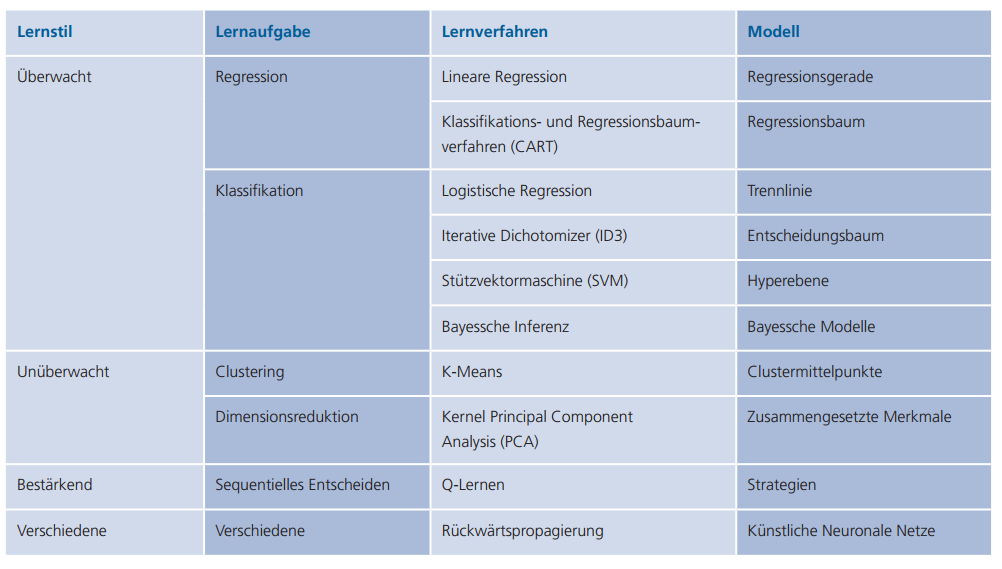
\includegraphics[width=0.9\textwidth]{images/lernverfahren}
	\caption{Gängige Lernverfahren und ihre Modelle \cite{Dobel.2018}}
	\label{fig:lernverfahren}
\end{figure}

Der Begriff des \textit{überwachten Lernens} inkludiert, dass während des Trainings bekannte (z.B. gemessene) Ausgangsgrößen dem System vorgegeben werden, um eine bestimmte Lernaufgabe (Klassifikation oder Regression) zu lösen. Nach dem Training des Netzes kann dann der Lernerfolg anhand bekannter richtiger Ergebnisse validiert und überwacht  werden. \\
Dagegen findet beim \textit{bestärkenden Lernen} keine direkte Übergabe der erwünschten Ausgabegrößen an das System statt. Stattdessen soll das System autonom eine Strategie erlernen, um die Anzahl der erhaltenen positiven Belohnungen zu maximieren. Dafür empfängt das System zu verschiedenen Zeitpunkten auf Basis seiner Aktionen eine positive oder negative Belohnung. Daraus ermittelt er eine Nutzenfunktion, welche seine Aktionen bewertet. Diese Nutzenfunktion entspricht üblicherweise seiner Strategie, die es zu verbessern gilt. \\
Beim \textit{unüberwachten Lernen} findet weder eine Übergabe der gewünschten Ausgangsgrößen noch eine Übergabe von Belohnungsanreizen an das System statt. Dieser Lernstil kommt somit vor allem bei Dimensionsreduktions- und Clustering-Anwendungen zum Einsatz. \\

Interessanterweise kommen neuronale Netze sowohl bei \textit{bestärkenden} (das Identifizieren einer Systemstrategie, um die Anzahl der empfangenen positiven Belohnungen zu maximieren) als auch bei \textit{überwachten} Lernstilen (zur Bildung eines nichtlinearen dynamischen Modells für ein System) zur Anwendung. Die Regelung der 3D-Servo-Presse kann prinzipiell durch das Anwenden beider Lernstile erfolgen, entweder durch das autonome Identifizieren einer Betriebsstrategie (das Einstellen der Spindel- und Exzentervorschübe), um die maximale Anzahl an positiven Belohnungen (das richtige Einstellen der Stößelposition) zu erreichen oder durch das Entwickeln eines nichtlinearen dynamischen Black-Box-Modells, welches als Hilfsglied in einem Regelkreis agiert oder in Kombination mit einem anderen Hilfsglied (welches ebenfalls ein neuronales Netz sein kann) selbst als Regler agiert.


%Für diese Arbeit stellt das überwachte Lernen das entscheidende Lernverfahren dar. Beim überwachten Lernen sind in den Trainingsdaten die Sollvorgaben in Form von gemessenen Ausgangsgrößen für die 3D-Servo-Presse (z.B. die Stößelhöhe) zu den korrespondierenden gemessenen Eingangsgrößen (Spindel- und Exzentervorschübe) vorhanden. Damit ist gewährleistet, dass das durch die Parametrisierung erzeugte Modell das Verhalten des realen Systems möglichst gut abbildet. \\
%Wie bereits erwähnt, gibt es im Bereich des überwachten Lernens zwei Anwendungsgebiete, zum einen die Klassifikation, zum anderen die Regression. Die gängigen Methode des maschinellen Lernens in diesen zwei Anwendungsgebieten sind in Tabelle \ref{tab:machine_learning} aufgelistet.

 

%Die Parametrisierung des Black-Box-Modells für die 3D-Servo-Pressen stellt eine Regressionsaufgabe dar. Dafür erscheint der Einsatz von neuronalen Netzen zweckmäßig.  






